\section{Možni načini uporabe spletnih portalov pri pouku}
\label{sec:načini_uporabe_sp}

V spodnjem sestavku izpostavimo nekatere skupne prednosti, ki jih
lahko prinese uporaba spletnih portalov za učenje programiranja pri
pouku. S pregledom spletnih portalov, ki so nastali na univerzah
(poglavje \ref{sec:SPUP}) in tistimi ki smo jih podrobno pregledali
(poglavje \ref{sec:pregled_spletnih_port}) lahko ugotovimo naslednje
prednosti.

\begin{description}
\tightlist
\item[Nepotrebna namestitev programske opreme] je zagotovo velika
  prednost. Mentorju praktično ni potrebno nameščati nobenega
  urejevalnika besedil, IDE, niti prevajalnika ali tolmača. Prav tako
  ni potrebe po nastavljanju sistemskih poti, ki jih mnogi
  prevajalniki zahtevajo. Uporaba SPUP je neodvisna od uporabe
  operacijskega sistema. Vsaka naprava, na kateri lahko poganjamo
  novodobni spletni brskalnik omogoča uporabo SPUP. Učencem na domačih
  računalnikih ni potrebno instalirati nobene programske opreme. Na
  tem mestu bi poudarili, da učitelj mora biti previden pri dajanju
  domače naloge z uporabo računalnika. Zares se mora prepričati, da to
  zmožnost imajo vsi učenci. Najbolje je da vso dodatno delo, ki ga
  učitelj predvidi lahko učenci opravijo v šolski računalniški
  učilnici.
\item[Seznanjanje s programsko opremo] pri pouku ni potrebno. Znebimo
  se potrebe, da bi z novinci morali spoznavati urejevalnik besedil
  ali kompleksno IRO. Spoznavanje programskega jezika in reševanje
  problemov se lahko lotijo nemudoma.
\item[Pisanje progama od začetka do konca] ni potrebno. Večina
  spletnih portalov, ki ponujajo vsebine v obliki vadnice, imajo
  programske naloge pripravljene tako, da uporabnik mora vnesti le del
  programske kode. Za novinca, to pomeni, da se osredotoči le na
  nalogo in del sintakse, ki jo v danem trenutku potrebuje, da reši
  zadano nalogo. To prednost smo že spoznali na SPUP avstralske
  univerze, kjer so uporabili, tip naloge, zapolni prazna mesta
  \cite{thesisAWebP}.
\item
\end{description}

Pripravili smo tudi konkretna primera, za OŠ in SŠ, kako bi s spletnim
portalom lahko uresničili učne cilje, ki jih najdemo v učnem načrtu.

\subsection{Primer uresničevanja ciljev učnega načrta v osnovni šoli}
\label{sec:uresn-cilj-unega-os}

V učnem načrtu Računalništvo - neobvezni izbirni predmet
\cite{ucni_nacrt-neobvezni-izbirni-os} vsebuje vsebinski sklop
\textbf{Algoritmi}, ki smo ga povzeli v poglavju
\ref{sec:neobvezno_izbirni_predmet_rac}. Spletni portal
\emph{\href{https://codecombat.com/}{Code combat}}
\cite{web:codecombat} lahko učitelj uporabi pri\textbf{ ponovitvi
  sklopa}, ko je snov že predelal na primer s programskim jezikom in
spletnim orodjem \emph{\href{https://scratch.mit.edu/}{Scratch}}
\cite{web:scratch}. K obstoječim ciljem, ki so podani v učnem načrtu
lahko dodamo še naslednje: \emph{učenci spoznajo osnove programskega
  jezika \textbf{Python}.}  Ker se učenci s pisanim programskim
jezikom srečujejo prvič bi bilo dobro, da učitelj pripravi učne liste
s primerjavo med \emph{Scratchom} in sintakso \textbf{Pythona}
oz. metodami, ki se uporabljajo na portalu (slika
\ref{fig:primerjava:cc01}). V tem primeru niti ni pomembno podrobna
obravnava programskega jezika Python. Pomembno je, da učenci razumejo
kaj posamezna vrstica programske kode izvrši, kateri del kode
predstavlja junaka in kateri akcijo junaka. To lahko pokažemo nazorno
z delom programske kode v \textbf{Scrach-u} (slika
\ref{fig:primerjava:scr01}), ki ponazarja metode, ki jih uporabljamo
na za vodenje junaka na spletni strani \emph{Comdecombat} (slika
\ref{fig:primerjava:cc01}).

 \begin{figure}[h!]
    \centering
    \begin{subfigure}[]{0.35\textwidth}
      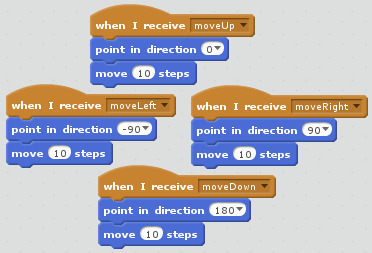
\includegraphics[width=\textwidth]{./images/sc_web/primerjava_scr-premiki-v01.jpg}
      \caption{Programska koda napisana v
        \emph{\href{https://scratch.mit.edu/}{Scratch-u}}
        \cite{web:scratch} za premikanje \emph{gor, levo, desno, dol}.}
        \label{fig:primerjava:scr01}
      \end{subfigure}
      \qquad
    \begin{subfigure}[]{0.35\textwidth}
        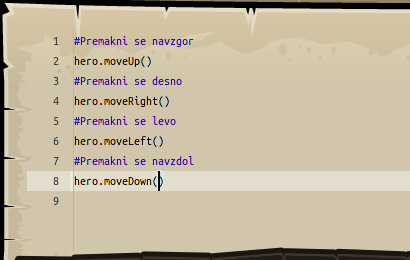
\includegraphics[width=\textwidth]{./images/sc_web/primerjava_cc-premiki-v01.jpg}
        \caption{Programska koda v \textbf{Pythonu} klica
          predpripravljene metode, ki premikajo junaka \emph{gor,
            levo, desno, dol}.}
          \cite{web:codecombat}
        \label{fig:primerjava:cc01}
    \end{subfigure}
    %Dodaj še za zanko
    % \\
    % \begin{subfigure}[]{0.25\textwidth}
    %   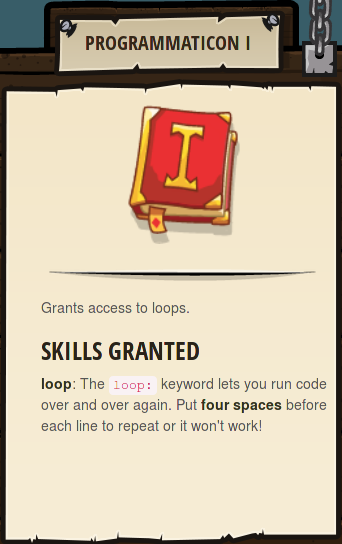
\includegraphics[width=\textwidth]{./images/sc_web/cc_EQ-P1-v01.png}
    %     \caption{Knjiga programiranja I}
    %     \label{fig:cc:eq:p1}
    %   \end{subfigure}
    %   \qquad
    % \begin{subfigure}[]{0.25\textwidth}
    %     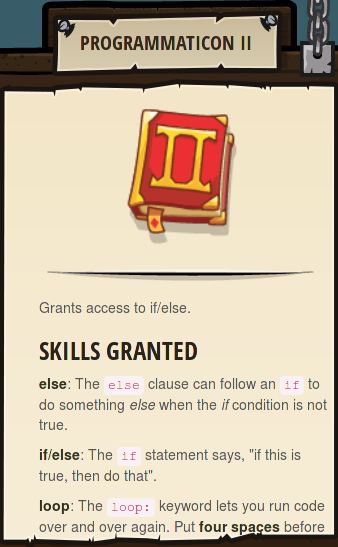
\includegraphics[width=\textwidth]{./images/sc_web/cc_EQ-P2-v01.png}
    %     \caption{Knjiga programiranja II}
    %     \label{fig:cc:eq:p2}
    % \end{subfigure}
    \caption{Primerjava programskih blokov napisanih v
      \textbf{Scratchu} in enačic klica metod napisanih v
      \textbf{Pythonu} na spletni strani \emph{Codecombat}}
   \label{fig:primerjava:scrVScc}
\end{figure} 

Kot smo že omenili v predstavitvi spletne ga portala \emph{Codecombat}
ima učitelj dve možnosti:

\begin{itemize}
\tightlist
\item učenci uporabljajo svoje ustvarjene račune,
\item učitelj ustvari \textbf{demo} razred in v njega vključi učence.
\end{itemize}

Glavna slabost v prvem primeru je ta, da tako lastno ustvarjeni računi
učencev omogočajo izbiro junakov, predmetov, ki jih uporabljajo pri
reševanju nalog in se zato lahko pri učni uri zaplete pri nadzoru
napredka pri posameznem učencu in je s tem delo učitelja oteženo. Iz
teh razlogov se raje nagibamo k drugi možnosti.

Učitelj lahko s prošnjo zaprosi \textbf{demonstracijski} račun v
katerem ima možnost, ustvariti razred s prvim vsebinskim sklopom
\textbf{Uvoda v računalniško znanost} (\emph{ang. Introduction to
  Computer Science }). To je edini sklop v tem načinu, ki je
brezplačen in ga lahko uporabimo v šoli pri nas brez dodatnih
stroškov. Učitelj učence povabi v razred z unikatno ustvarjenim
\textbf{URL} naslovom. Registracija po kliku na povezavo je potrebna.
Učenci se od naloge do naloge premikajo brez povzetka prejema dosežkov
in izbire predmetov in izbire opreme za svojega junaka.  Za tako delo
je primeren tip učen ure \textbf{praktično vodeno delo}, kjer učitelj
delo vodi z vnaprej pripravljenimi učnimi listi primerjave programskih
blokov (slika \ref{fig:primerjava:scrVScc}) in povzetki navodil v
slovenščini. Ko učenci v začetnih nalogah osvojijo osnovne metode
junaka lahko učitelj stopnjuje samostojnost dela učencev. Delo na
spletnem portalu je primerno za dvojno učno uro
oz. \textbf{90min}. Tiste naloge, ki jih učenci ne uspejo dokončati,
jih lahko učitelj da kot domače delo.

Sklop vsebinsko predstavlja naslednje koncepte programiranja
\textbf{osnove sintakse, argumenti, spremenljivke, tip
  spremenljivke:\texttt{string}, \texttt{while} zanka}. Pri
preverjanju sklopa nekatere operativne cilje ne moremo preveriti,
zapisali smo tiste, ki jih ni moč preveriti in zakaj.

\begin{itemize}
\tightlist
\item \textbf{algoritem predstavijo simbolno (z diagramom poteka) ali s
  pomočjo navodil v preprostem jeziku}. Na spletni strani algoritmi
niso predstavljeni z diagrami, lahko jih sicer pripravi učitelj,
vendar v tej fazi to ni nujno potrebno. 
\item \textbf{znajo v algoritem vključiti vejitev}. Uporaba vejitev v
  tem prvem sklopu \textbf{CS1} na spletnem portalu ni omogočena.
\item \emph{znajo uporabiti nekatere ključne algoritme za sortiranje in
  iskanje},
\item \emph{poznajo osnovne algoritme za iskanje podatkov}.
\end{itemize}

Menimo, da ostale cilje lahko uspešno povzamemo in preverimo v učni
uri ponovitve vsebinskega sklopa. Čeprav uporaba spletne igre
predstavlja kar nekaj priprave učitelja ima izjemno motivacijsko
vrednost, ki učence lahko navduši za nadaljnje delo. 

\subsection{Primer uresničevanja ciljev učnega načrta v srednji šoli}
\label{sec:prim-uresn-cil-ss}

Učni načrt \textbf{informatike} na programu Splošna gimnazija
predvideva učenje algoritmov in programiranja pa ravni
\textbf{posebnih znanj} v tematskem sklopu obdelave
podatkov. Predpostavimo, da mentor oz. profesor predmeta Informatika,
uresničuje znanja algoritmov in programiranja, ta lahko uporabi
spletni portal \emph{\href{https://www.codecademy.com/}{Codeacademy}}
\cite{web:codeacademy} v namene domačega dela. Profesor mora
upoštevati med predmetno povezovanj s predmetom angleščina in za dani
sklop pripraviti prevode navodil, ki so lahko dijakom v
pomoč. Prednost portala je še ta, da vsebinski sklopi in posamezne
teme, ki so na voljo, lahko poljubno izbiramo ne glede na vrstni red
oz. na to kaj smo že predelali. Kako lahko profesor izkoristi uporabo
sledenju napredka dijakov smo že podrobno opisali v poglavju
\ref{sec:uporaba_učitelji}.

Spletni portal lahko uporabi pred obravnavo neke snovi in se tako
dijaki že seznanijo z določeno funkcionalnostjo in sintakso
programskega jezika. Ker dijaki že del znanja in sintakse usvojijo so
naloge pri pouku lahko zahtevnejše in je lahko večji poudarek na
strategiji reševanja (težjih) problemov. Konkretno, za domače delo
lahko dijaki rešujejo nalogo \emph{``Strings \& Console Output''}, kjer
osvojijo osnovno znanje ravnanja z \textbf{pisanjem izhodnih podatkov}
in \textbf{podatkovnega tipa \texttt{string} oz. \texttt{niza}}. Naučijo se
uporabljati metode, ki jih ponuja podatkovni tip \texttt{string},
lepijo dve besedi skupaj in tako dalje. Kot že reženo, z osvojenim
znanjem pozneje pri pouku lahko rešujejo zahtevnejše naloge.

V drugem primeru lahko ta isti portal uporabi po obravnavi določenega
vsebinskega sklopa in vadnico na portalu
\emph{\href{https://www.codecademy.com/}{Codeacademy}}
\cite{web:codeacademy} izkoristi, dijaki z domačim delom utrdijo svoje
znanje. Poglejmo konkreten primer.  Dijaki na primer po
\textbf{obravnavi sklopa, vhodni podatki, podatkovni tip,
  \texttt{string}} in \textbf{\texttt{if else} vejitve}, imajo
zadostno znanje da rešijo nalogo \emph{``PygLatin''}. Napisati morajo
program, ki sprejme besedo in jo pretvori po določenem pravilu
slovarja ter jo izpiše na zaslon. Naloga je razdeljena na več vadnic,
dijaki tako postopno rešujejo korak po koraku nalogo. Napredek
reševanja naloge lahko spremlja profesor preko portala.

  %%% Local Variables:
  %%% mode: latex
  %%% TeX-master: "../diploma"
  %%% End:
